\section{Appendix B}
\label{app:simulations}
\subsection{SPI In}

\begin{figure}[H]
  \centering
  \captionsetup{justification=centering}
  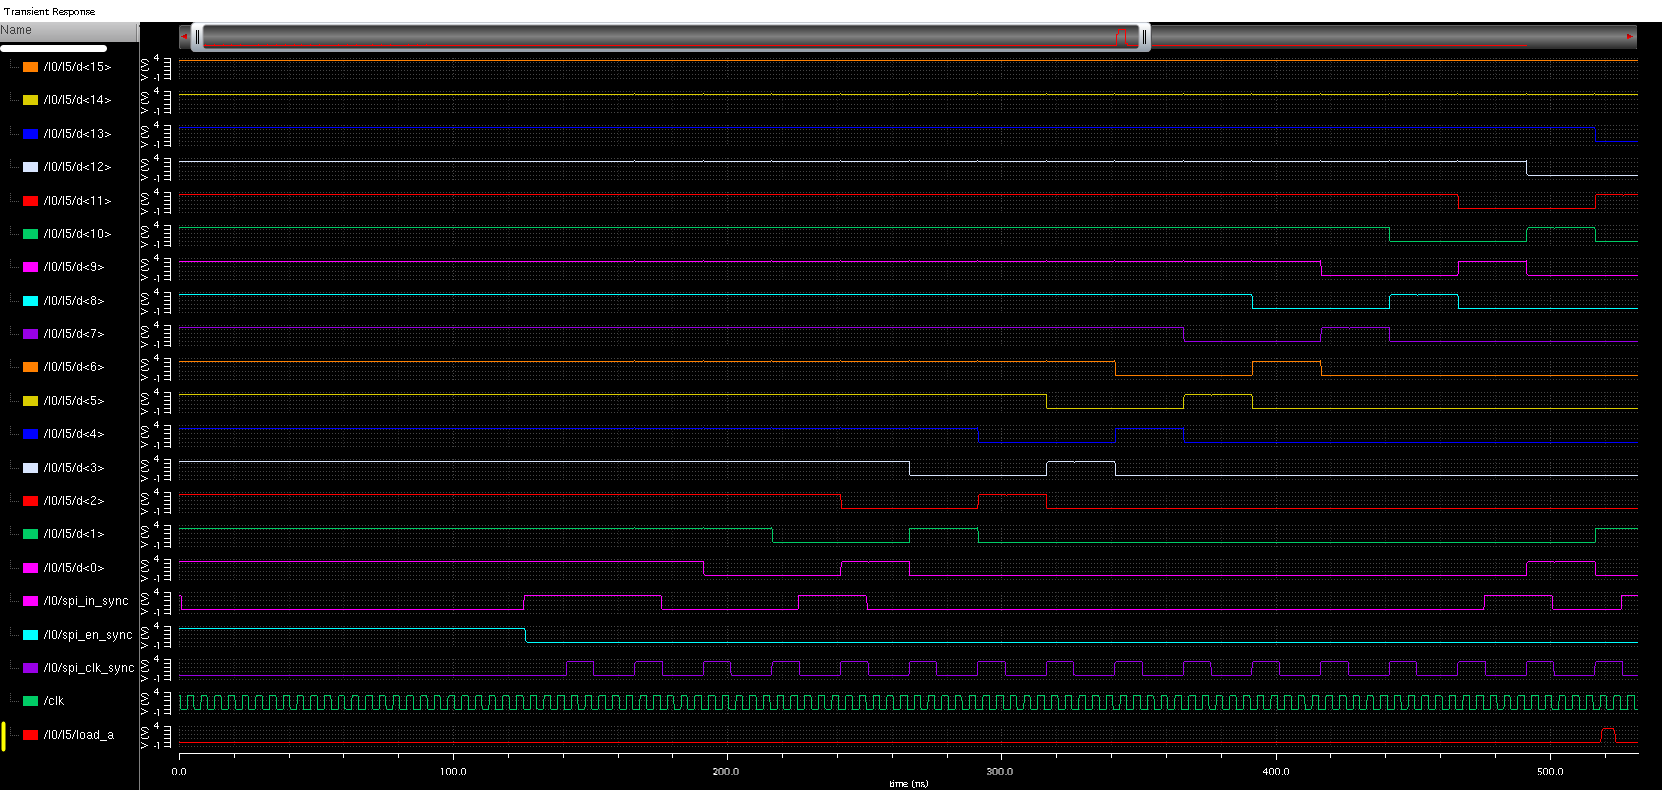
\includegraphics[angle=90, scale=0.44]{../figures/test2_spi_in}
  \caption{SPI receiver} 
\end{figure}

\begin{figure}[H]
  \centering
  \captionsetup{justification=centering}
  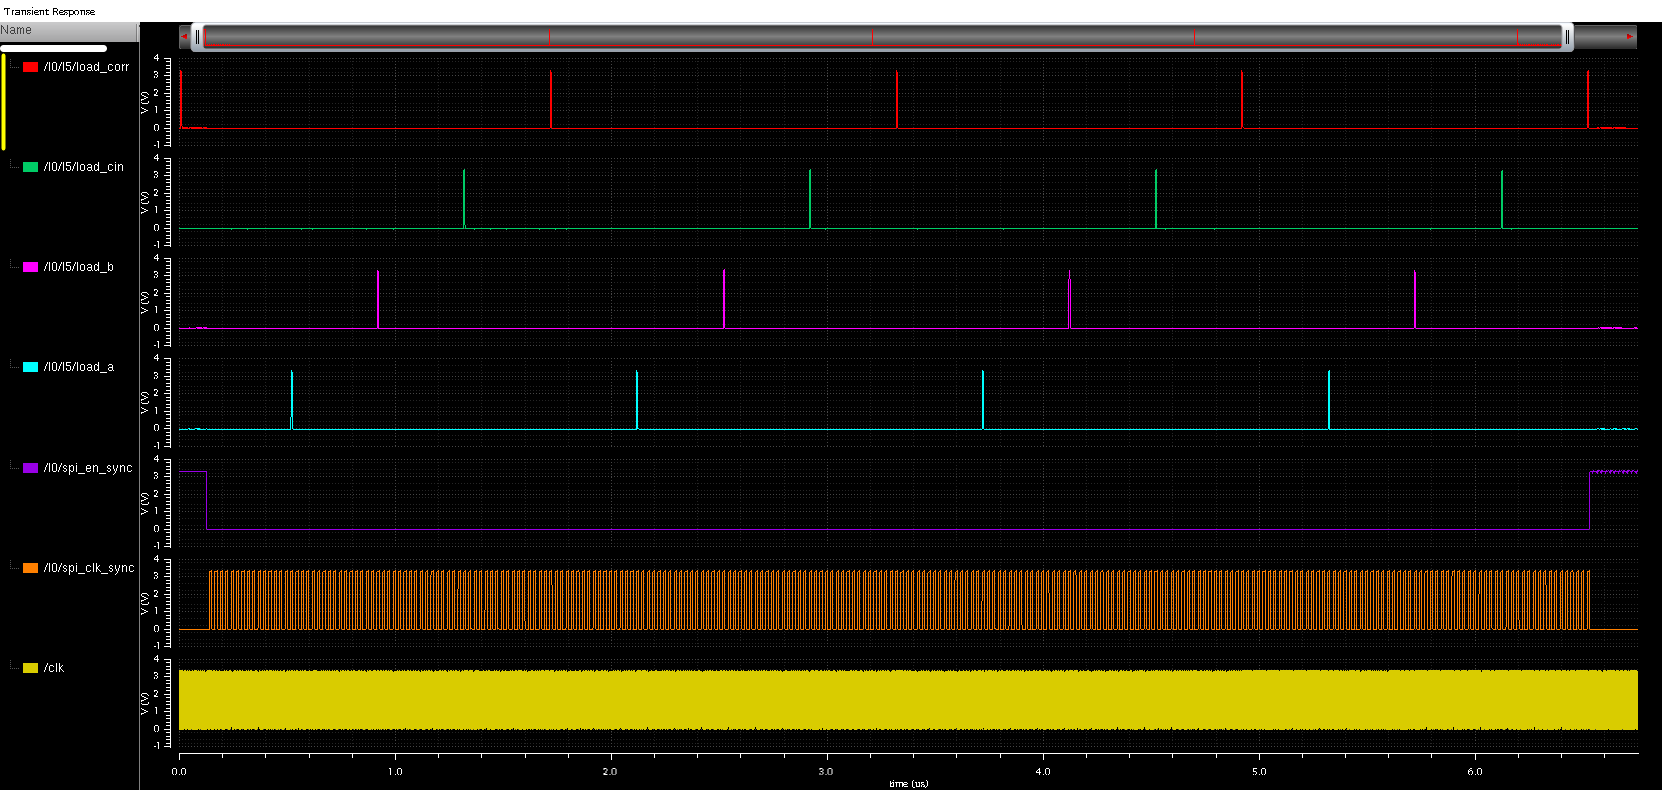
\includegraphics[angle=90, scale=0.46]{../figures/test2_spi_load}
  \caption{Load signals}
\end{figure}

\begin{figure}[H]
  \centering
  \captionsetup{justification=centering}
  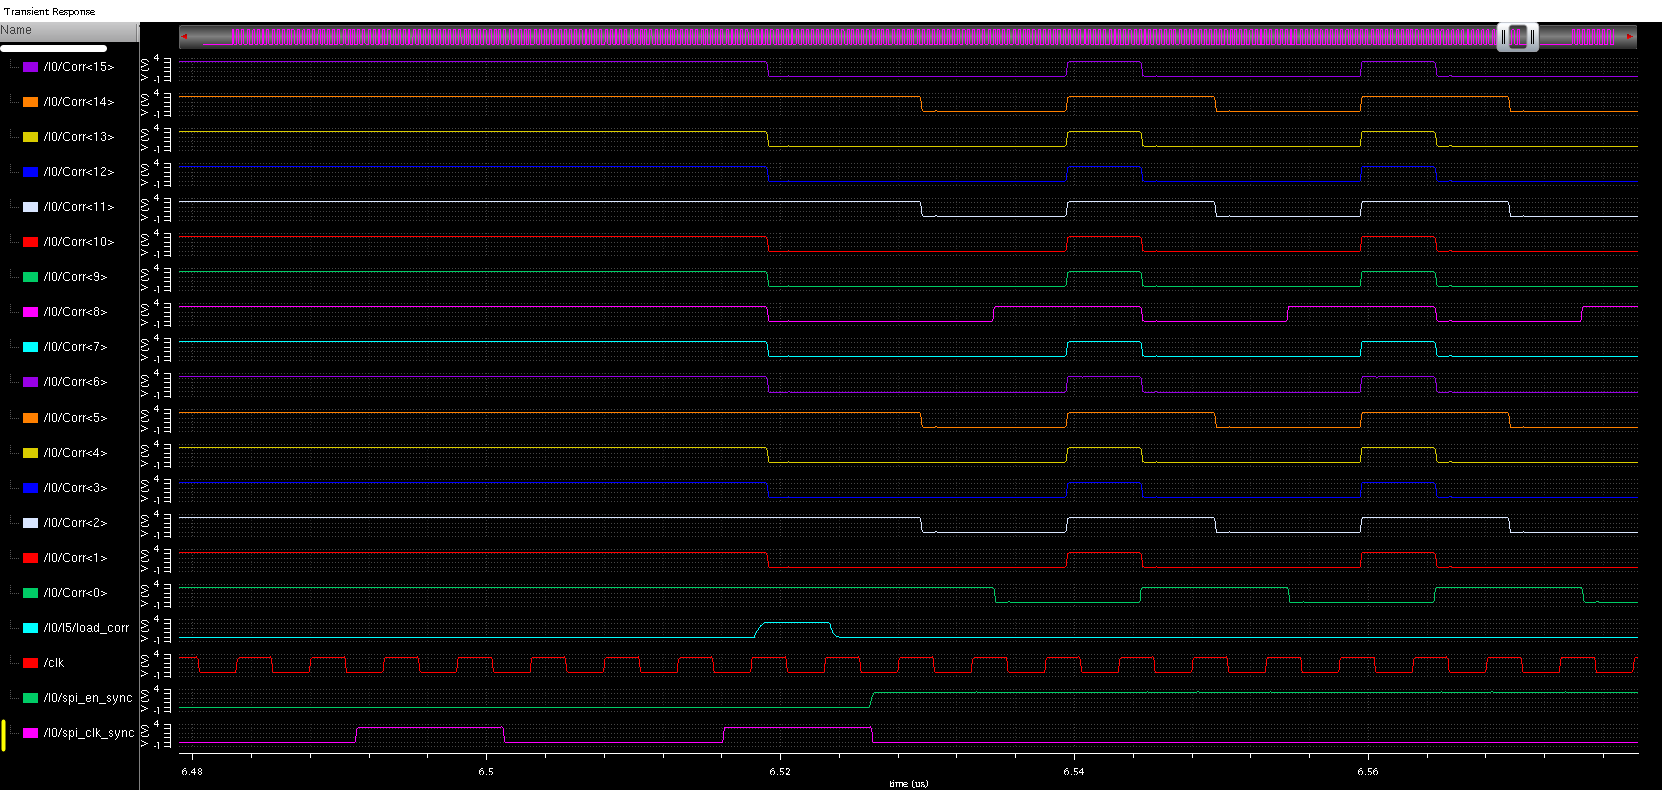
\includegraphics[angle=90, scale=0.46]{../figures/test2_spi_abc}
  \caption{PRBS registers}
\end{figure}

\subsection{SPI Out}

\begin{figure}[H]
  \centering
  \captionsetup{justification=centering}
  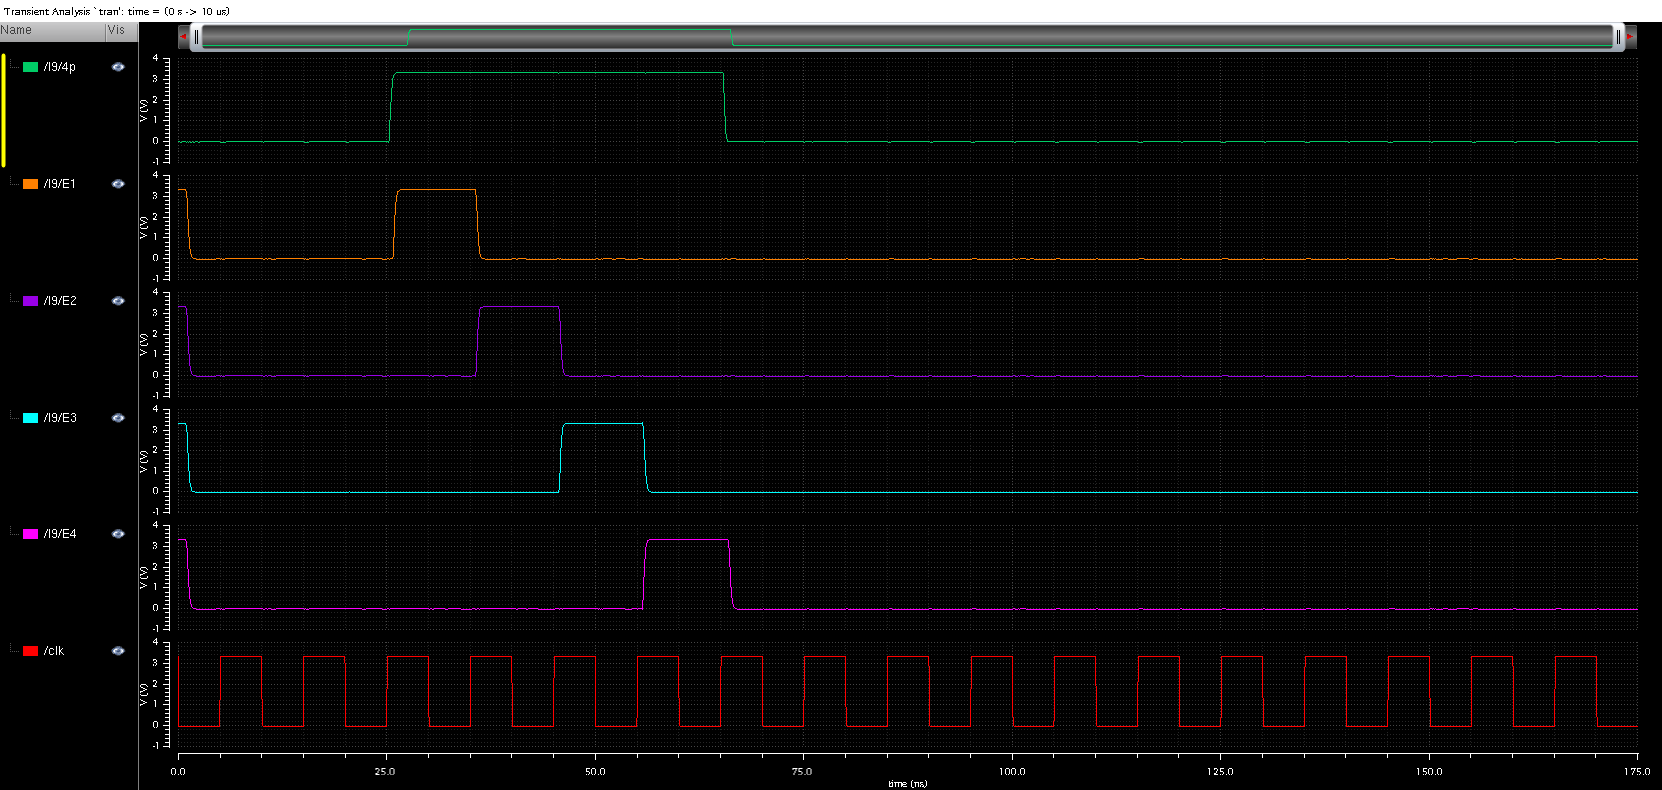
\includegraphics[angle=0, scale=0.55]{../figures/spi_out_control}
  \caption{Enable high} \label{fig:spi_out1}
\end{figure}

\begin{figure}[H]
  \centering
  \captionsetup{justification=centering}
  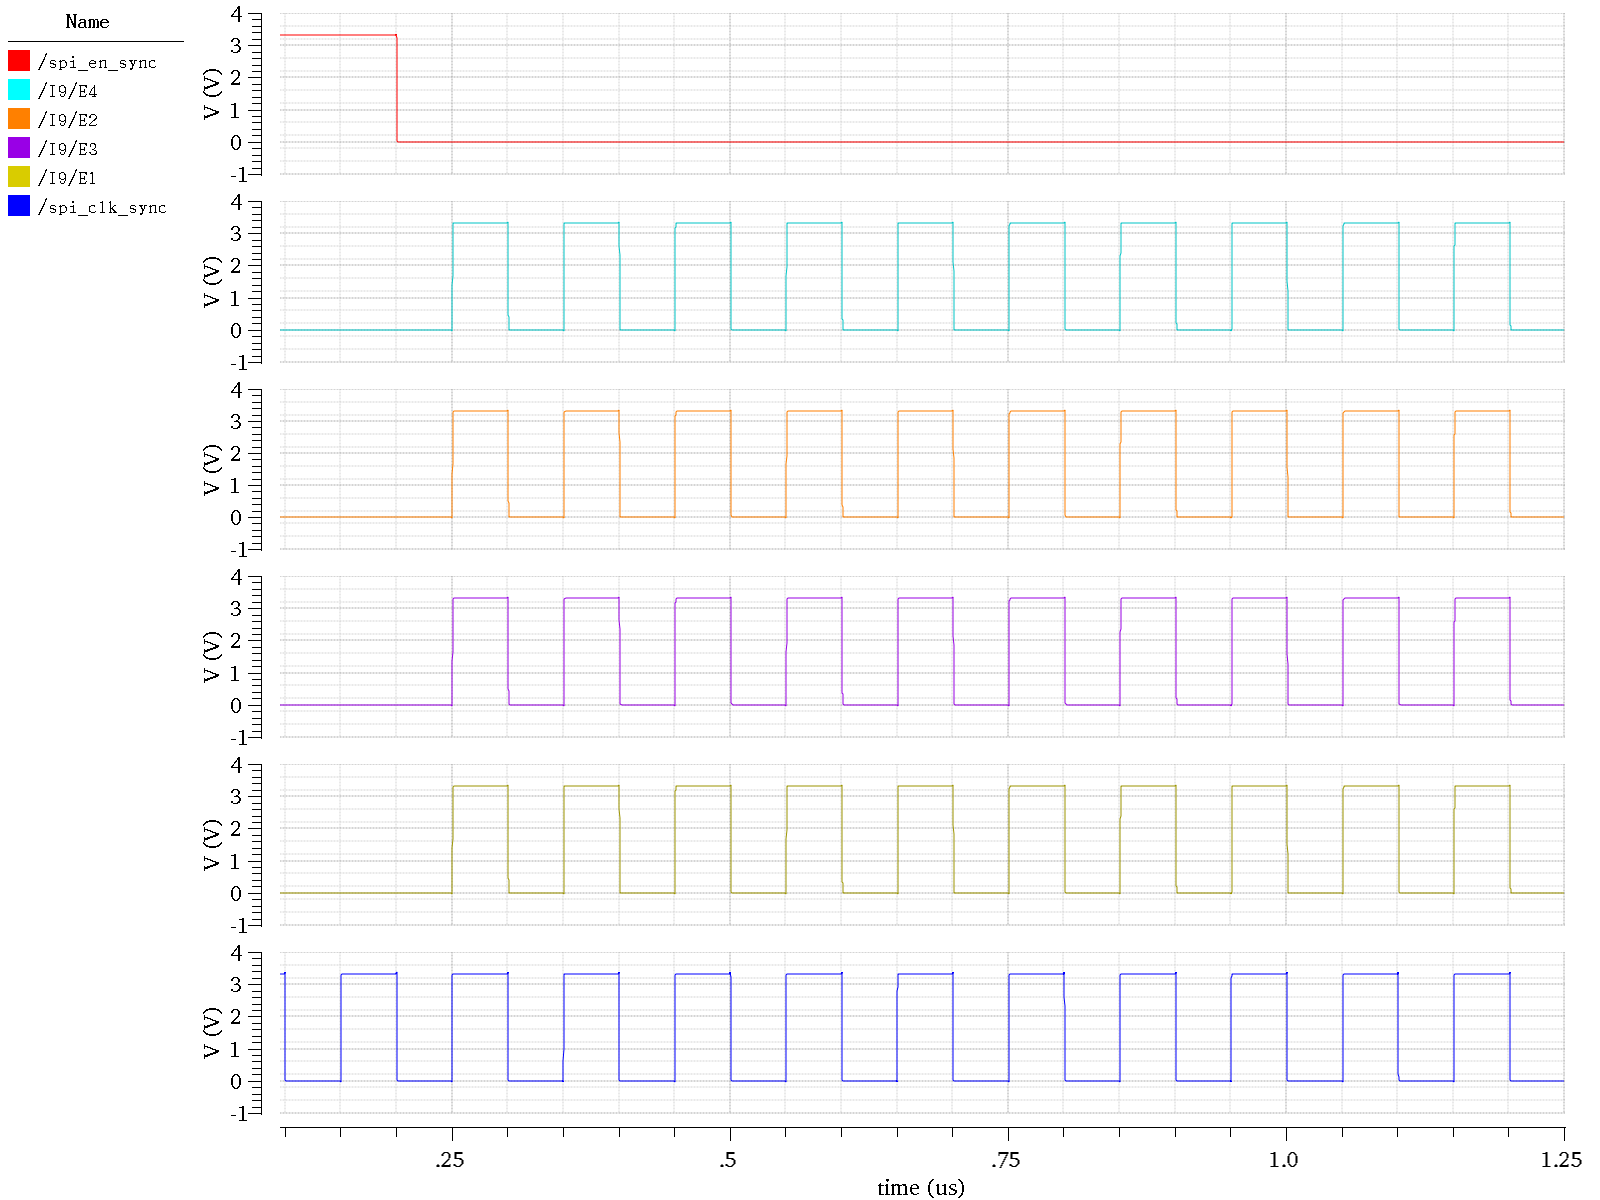
\includegraphics[angle=0, scale=0.55]{../figures/spi_out_control2}
  \caption{Enable low} \label{fig:spi_out2}
\end{figure}

\subsection{Adder}

\begin{figure}[H]
  \centering
  \captionsetup{justification=centering}
  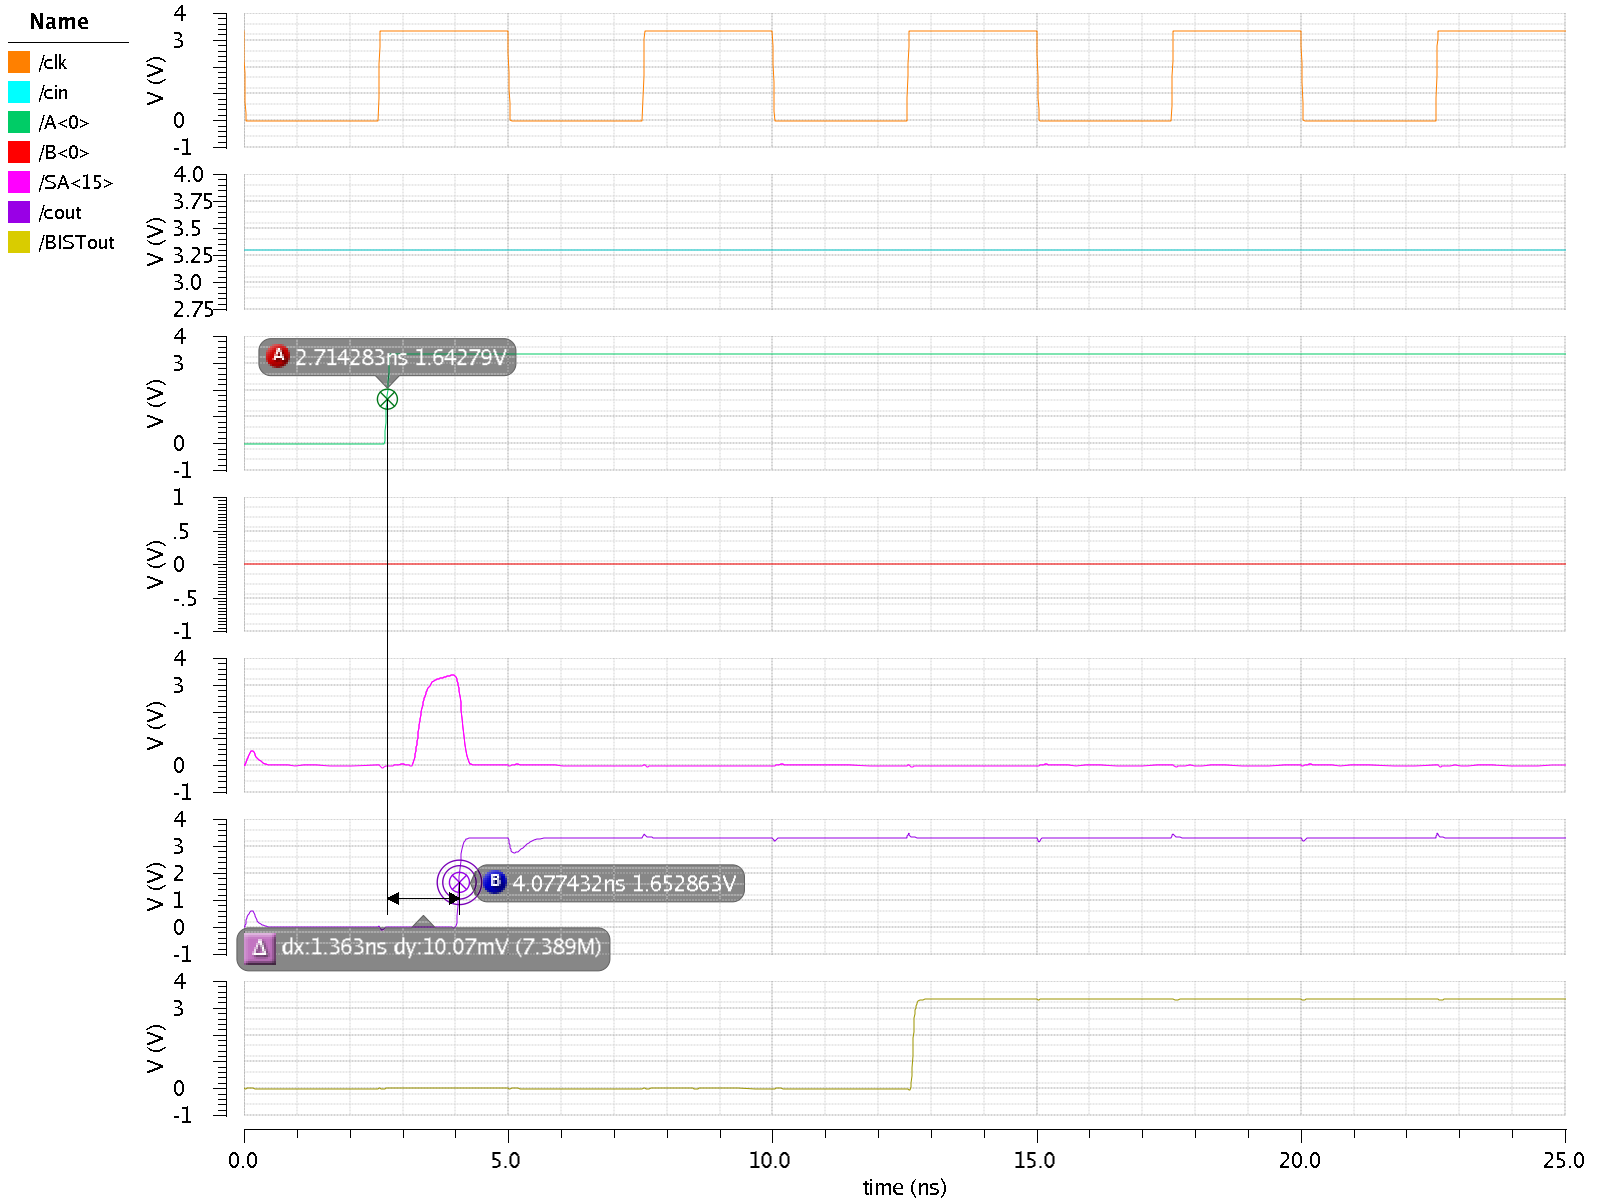
\includegraphics[angle=90, scale=1]{../figures/kogge_delay}
  \caption{Worst case propagation delay Kogge-Stone Adder} \label{fig:kogge_delay}
\end{figure}

